%%%%%%%%%%%%%%%%%%%%%%%%%%%%%%%%%%%%%%%%%
% Short Sectioned Assignment LaTeX Template Version 1.0 (5/5/12)
% This template has been downloaded from: http://www.LaTeXTemplates.com
% Original author:  Frits Wenneker (http://www.howtotex.com)
% License: CC BY-NC-SA 3.0 (http://creativecommons.org/licenses/by-nc-sa/3.0/)
%%%%%%%%%%%%%%%%%%%%%%%%%%%%%%%%%%%%%%%%%

%----------------------------------------------------------------------------------------
%	PACKAGES AND OTHER DOCUMENT CONFIGURATIONS
%----------------------------------------------------------------------------------------

\documentclass[paper=a4, fontsize=11pt]{scrartcl} % A4 paper and 11pt font size

% ---- Entrada y salida de texto -----

\usepackage[T1]{fontenc} % Use 8-bit encoding that has 256 glyphs
\usepackage[utf8]{inputenc}
%\usepackage{fourier} % Use the Adobe Utopia font for the document - comment this line to return to the LaTeX default

% ---- Idioma --------

\usepackage[spanish, es-tabla]{babel} % Selecciona el español para palabras introducidas automáticamente, p.ej. "septiembre" en la fecha y especifica que se use la palabra Tabla en vez de Cuadro

% ---- Otros paquetes ----

\usepackage{amsmath,amsfonts,amsthm} % Math packages
%\usepackage{graphics,graphicx, floatrow} %para incluir imágenes y notas en las imágenes
\usepackage{graphics,graphicx, float, url} %para incluir imágenes y colocarlas

% Para hacer tablas comlejas
%\usepackage{multirow}
%\usepackage{threeparttable}
\usepackage{float}


%\usepackage{sectsty} % Allows customizing section commands
%\allsectionsfont{\centering \normalfont\scshape} % Make all sections centered, the default font and small caps

\usepackage{fancyhdr} % Custom headers and footers
\pagestyle{fancyplain} % Makes all pages in the document conform to the custom headers and footers
\fancyhead{} % No page header - if you want one, create it in the same way as the footers below
\fancyfoot[L]{} % Empty left footer
\fancyfoot[C]{} % Empty center footer
\fancyfoot[R]{\thepage} % Page numbering for right footer
\renewcommand{\headrulewidth}{0pt} % Remove header underlines
\renewcommand{\footrulewidth}{0pt} % Remove footer underlines
\setlength{\headheight}{13.6pt} % Customize the height of the header

\numberwithin{equation}{section} % Number equations within sections (i.e. 1.1, 1.2, 2.1, 2.2 instead of 1, 2, 3, 4)
\numberwithin{figure}{section} % Number figures within sections (i.e. 1.1, 1.2, 2.1, 2.2 instead of 1, 2, 3, 4)
\numberwithin{table}{section} % Number tables within sections (i.e. 1.1, 1.2, 2.1, 2.2 instead of 1, 2, 3, 4)

\setlength\parindent{0pt} % Removes all indentation from paragraphs - comment this line for an assignment with lots of text

\newcommand{\horrule}[1]{\rule{\linewidth}{#1}} % Create horizontal rule command with 1 argument of height


\title{	
	\normalfont \normalsize 
	\textsc{{\bf Ingeniería de Servidores (2015-2016)} \\ Grado en Ingeniería Informática y Matemáticas \\ Universidad de Granada} \\ [25pt] % Your university, school and/or department name(s)
	\horrule{0.5pt} \\[0.4cm] % Thin top horizontal rule
	\huge Memoria Práctica 3 \\ % The assignment title
	\horrule{2pt} \\[0.5cm] % Thick bottom horizontal rule
}

\author{Iván Sevillano García} % Nombre y apellidos

\date{\normalsize\today} % Incluye la fecha actual

\begin{document}

\maketitle % Muestra el Título

\newpage %inserta un salto de página

\tableofcontents % para generar el índice de contenidos

\newpage

\section{Conociendo el subsistema de archivos.}

\subsection{Cuestión 1:}

\begin{itemize}
	\item \textbf{¿Qué archivo le permite ver qué programas se han instalado con el gestor de paquetes?}\\
	En el directorio $/var/log/apt/$,donde se encuentran los archivos history.log y term.log. Además, encontramos también archivos con los mismos nombres con las extensiones que abajo se especifican(donde podemos encontrar cualquier número como extensión).
	
	\item \textbf{¿Qué significan las terminaciones .1.gz o .2.gz de los archivos en ese directorio?}\\
	Cada vez que llenamos lo suficiente nuestro archivo history.log, el sistema la comprime y crea un nuevo history.log para almacenar la información sobre nuevos paquetes que instalemos. Las extensiones con distinto número no son más que formas de numerar los distintos paquetes por orden. El orden que siguen va desde el más reciente (extensión .1.gz) hasta el más antiguo.
	
\end{itemize}

\subsection{Programación de tareas con cron}
\begin{itemize}
	\item \textbf{¿Qué archivo ha de modificar para programar una tarea? Escriba la línea
		necesaria para ejecutar una vez al día una copia del directorio ~/codigo a ~/seguridad/
		$fecha$ donde $fecha$ es la fecha actual (puede usar el comando date)}\\
	Según \cite{crontab}, debemos modificar los archivos en $/var/spool/cron/crontabs/$, sin embargo no están hechos para ser modificados directamente. Se nos ofrece, para modificar el archivo de programación de tareas, el comando $crontab$, que con la opción $-e$, nos deja modificar desde la terminal con el editor de texto que prefiramos.\\
	
	La linea que debemos añadir será la siguiente:\\
	
	$0 0 * * * cp -r ~codigo ~/seguridad/`date`$\\
	
	Los primeros cinco $items$ de la sentencia indican cuando queremos que se realice la tarea que se muestra a continuación, por este orden: minuto hora diaDelMes Mes DiaDeLaSemana. No hace especificar todos los campos, ya que el poner un asterisco($*$) nos dice que no tenga en cuenta este campo. Por ello, en nuestra sentencia, queremos que se ejecute el comando siempre que sean las doce de la noche, sea el día que sea, el mes que sea y el día de la semana que sea.
\end{itemize}

\section{Analizando que ocurre en el Kernel con Dmesg}

\begin{itemize}
	\item \textbf{Pruebe a ejecutar el comando, conectar un dispositivo USB y vuelva a
		ejecutar el comando. Copie y pegue la salida del comando (considere usar dmesg |
		tail). Comente qué observa en la información mostrada.}\\
	
	\begin{figure}[H]
	\centering
	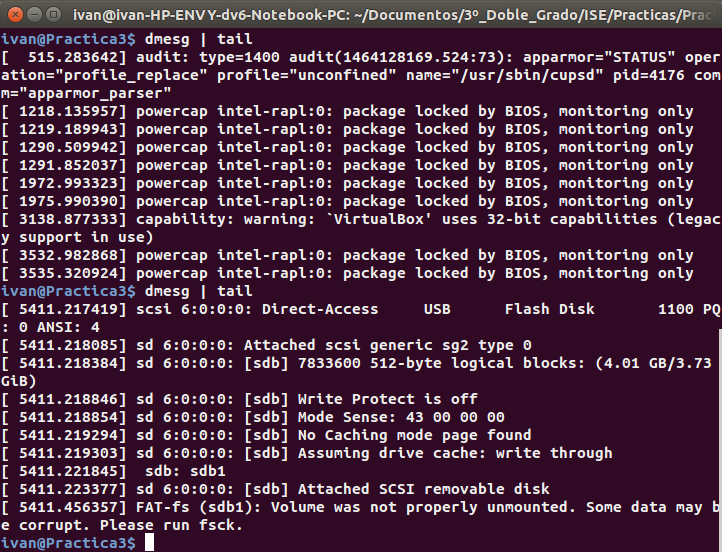
\includegraphics[width=0.7\linewidth]{dmesgPenDrive}
	\caption[dmesg]{Mensaje mostrado por dmesg antes y después de conectar un pen-drive}
	\label{fig:dmesgPenDrive}
	\end{figure}
	
	Antes de conectar el pen-drive, no teníamos ninguna referencia del mismo. Tras conectarlo, el primer mensaje que se nos muestra es la presencia del mismo. También nos ofrece más información como que el disco no fue debidamente desmontado.

	
\end{itemize}

\section{Monitorización del Hardware.}

\begin{itemize}
	\item \textbf{Instale alguno de los monitores comentados arriba en su máquina y
		pruebe a ejecutarlos (tenga en cuenta que si lo hace en la máquina virtual, los
		resultados pueden no ser realistas). Alternativamente, busque otros monitores para
		hardware comerciales o de código abierto para Windows y Linux.}\\
	El primer monitor instalado en el sistema de $hddtemp$ \cite{hddtemp}, que nos muestra la temperatura de los discos duros de nuestro PC en Linux. Tras ejecutar $hddtemp$ sobre un disco duro en concreto(En nuestro caso $/dev/sda$), nos puede salir una salida como la siguiente:\\
	
	$/dev/sda:$ $ST500LM012$ $HN-M500MBB:$ $48ºC$\\
	
	en el cual nos muestra que la temperatura del mismo es 48 grados celsius. Mas información en el manual, antes citado.\\
	
	Para detectar los sensores de la placa base necesitamos instalar la librería $lm-sensors$ \cite{sensors}(la página del proyecto está caida). Esta librería es necesaria para el siguiente monitor gráfico del sistema, psensor, que se instala con el paquete del mismo nombre. Este monitor nos ofrece de forma gráfica la información sobre temperatura y porcentaje de la CPU usado. Un ejemplo de la interfaz es la siguiente:\\
	
	\begin{figure}[H]
	\centering
	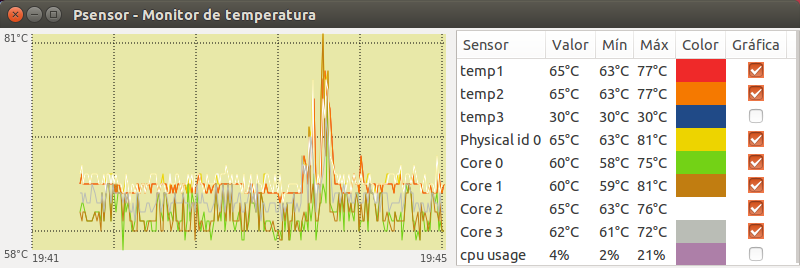
\includegraphics[width=0.7\linewidth]{psensor}
	\caption[psensor]{Gráfica que muestra psensor sobre la temperatura de algunos componentes del sistema.}
	\label{fig:psensor}
	\end{figure}
	
	Además de estos, se pueden encontrar en \cite{HWMon} otras herramientas de monitorización, como por ejemplo Hardinfo\cite{hardinfo}, que es una aplicación libre la cual muestra información acerca de los distintos componentes del sistema como el procesador, distintos dispositivos como USB's, o incluso realizar benchmarking sobre los mismos.\\
	
	
	En Windows\cite{WMonitor}, algunas de las herramientas que podemos usar para monitorizar el sistema en lugar de las ya dadas son las siguientes, entre otros:\\
	\begin{itemize}
		\item Prime95\cite{prime95}, que se encarga de cargar de trabajo todos los núcleos para comprobar su rendimiento.
		\item MemTest86\cite{memtest86}, utilizado para testear la memoria RAM.
	\end{itemize}
\end{itemize}

\section{Otros monitores de sistema.}
\subsection{Munin}
\begin{itemize}
	\item \textbf{Visite la web del proyecto y acceda a la demo que proporcionan(http://demo.munin-monitoring.org/) donde se muestra cómo monitorizan un servidor. Monitorice varios parámetros y haga capturas de pantalla de lo que está mostrando comentando qué observa.}
	
	El primer parámetro que vamos a monitorizar es el uso de la CPU. La siguiente imagen nos dice cual es el porcentaje usado por distintos consumidores al día:\\
	
	\begin{figure}[H]
	\centering
	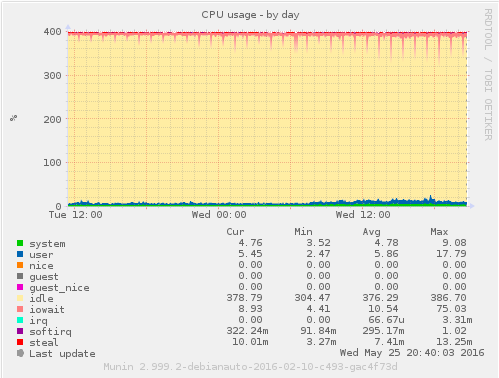
\includegraphics[width=0.7\linewidth]{monitoring_munin_cpu}
	\caption[CPUusage]{Uso de la CPU durante un día en el servidor que monitoriza Munin}
	\label{fig:monitoring_munin_cpu}
	\end{figure}
	
	Otro parámetro a monitorizar que nos ofrece Munin es el número de procesos y el estado de los mismos:\\
	
	\begin{figure}[H]
	\centering
	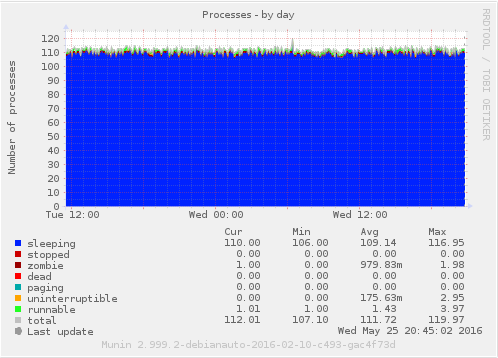
\includegraphics[width=0.7\linewidth]{monitorin_munin_procesos}
	\caption[ProcesosMunin]{Número de procesos y estado de los mismos.}
	\label{fig:monitorin_munin_procesos}
	\end{figure}
	
	En este gráfico vemos que hay alrededor de 110 procesos lanzados de los cuales la gran mayoría está $sleeping$, o esperando a estar corriendo. También vemos que apenas han quedado procesos zombies. Es importante notar que siempre hay al menos un proceso ejecutandose.
	
\end{itemize}
\subsection{Nagios}
\begin{itemize}
	\item \textbf{Instale Nagios en su sistema (el que prefiera) documentando el
		proceso y muestre el resultado de la monitorización de su sistema comentando qué
		aparece.}
	Para instalar Nagios por medio de la herramienta apt, ejecutamos el siguiente comando:\\
	
	$sudo$ $apt-get$ $install$ $nagios3$\\
	
	Tras esto, en el proceso de instalación nos preguntan que configuración deseamos, en nuestro caso la que esté por defecto:\\
	\begin{figure}[H]
	\centering
	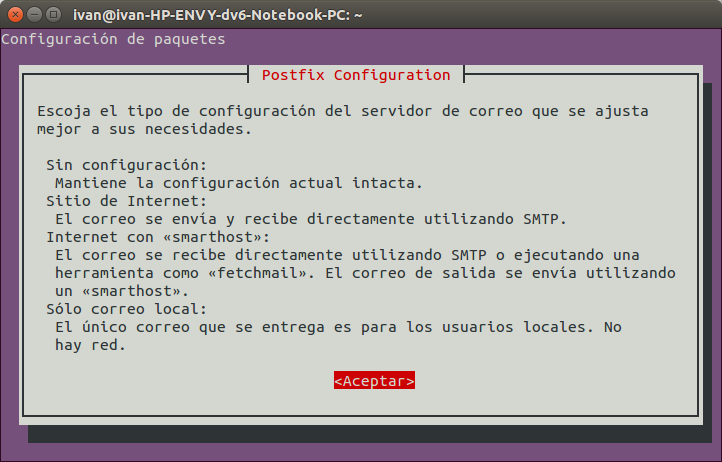
\includegraphics[width=0.7\linewidth]{Nagios1}
	\caption[Configuración]{Configuraciones posibles de Nagios.}
	\label{fig:Nagios1}
	\end{figure}
	
	También nos pide un nombre de dominio:\\
	\begin{figure}[H]
	\centering
	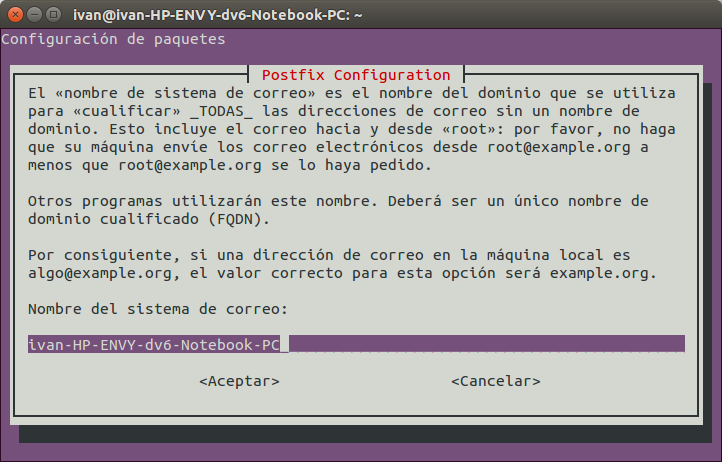
\includegraphics[width=0.7\linewidth]{Nagios2}
	\caption[nagios2]{Solicitud de nombre de dominio.}
	\label{fig:Nagios2}
	\end{figure}
	
	También nos pide una contraseña para Nagios.
	
\end{itemize}

\subsection{Monitorizando un servicio}
\begin{itemize}
	\item \textbf{Escriba un breve resumen sobre alguno de los artículos donde se muestra
		el uso de strace, o busque otro programa similar y coméntelo.}\\
	
	En mi caso, he visitado la página\cite{strace}, en la que se habla de algunas utilidades de strace y de un problema que el escritor solucionó gracias a este monitor de servicios. Las primeras líneas nos explican que esta herramienta no solo puede monitorizar un servicio desde el principio (lanzándolo con strace), si no que también puede lanzarse aunque el servicio ya esté ejecutándose. Esto es muy útil a la hora de monitorizar daemons que no deban ser reiniciados muy a menudo. En cuanto al problema que plantea, se resume de la siguiente manera: Se está utilizando un servicio SVN que fallaba aleatoriamente y nadie podía acceder al mismo. Reiniciar el servidor arreglaba el problema, pero no permanentemente, volvía a fallar. Al escritor se le ocurrió buscar en los archivos log, pero no había ninguno. Además, a la hora de observar cómo se iniciaban los procesos, todo parecía correcto, pero por alguna razón, el sistema se colgaba. Entonces recurrió, puesto que no podía modificar el código con opciones de debugueo, a utilizar un script que lanzara svnserver pero cazando la información que nos pueda dar strace. De esta forma, los clientes podrían seguir utilizando el servicio. Este cambio hizo visible el problema fácilmente en cuanto varios usuarios utilizaron el servicio. El problema era que a la hora de dar $filehandle$ para lectura, se daba el filehandle número 5, pero este fallaba. \\
	
	Por lo visto, este problema ocurre cuando el sistema no tiene la suficiente entropía para generar un stream aleatorio, por lo que reiniciar el sistema podría solucionar parcialmente el problema(podría "reiniciar" la entropía). El por qué de esta falta de entropía no se aclara ya que, según el autor, no era necesario. Utilizando, en vez de el generador de streams aleatorios $/dev/random$, otro generador que no fallase con la falta de entropía, $/dev/urandom$ , solucionó fácilmente el problema. En principio esto es un fallo de seguridad, pero en el trabajo que estaban realizando y según el criterio del autor, este fallo era irrelevante.\\
	
	La entrada del blog termina diciendo que este problema hubiese sido imposible de resolver sin un debugger o strace, siendo este último bastante más sencillo de utilizar.
	
\end{itemize}

\section{Profiling}

\subsection{Bases de datos}

\begin{itemize}
	\item \textbf{Acceda a la consola mysql (o a través de phpMyAdmin) y muestre el
		resultado de mostrar el ”profile” de una consulta (la creación de la BD y la consulta la
		puede hacer libremente)}\\
	
\end{itemize}
\newpage
\begin{thebibliography}{xx}
	\bibitem{crontab} http://linux.die.net/man/1/crontab
	\bibitem{hddtemp} http://linux.die.net/man/8/hddtemp
	\bibitem{sensors} http://www.tecmint.com/psensor-monitors-hardware-temperature-in-linux/
	\bibitem{HWMon} http://www.educadictos.com/herramientas-de-monitorizacion-de-hardware-para-ubuntu-12-04/
	\bibitem{hardinfo} http://www.guia-ubuntu.com/index.php/HardInfo
	\bibitem{WMonitor} http://hardzone.es/programas-para-testear-monitorizar-y-comprobar-el-rendimiento-de-tu-pc/
	\bibitem{prime95} http://www.mersenne.org/
	\bibitem{memtest86} http://www.memtest86.com/
	\bibitem{nagios} https://www.nagios.org/
	\bibitem{strace} https://debian-administration.org/article/352/Using_strace_to_debug_application_errors
	
\end{thebibliography}
\end{document}